\documentclass[10pt,dvipdfm]{beamer}

\usepackage{hcystyle}

%%%%%%%文档正文
\begin{document}

%标题作者等信息。
%这些信息将自动生成ppt的第一页
\title[毕业设计答辩]{\LARGE{
			基于动态链接技术的web服务器动态扩展功能
				接口的设计与实现
	}}
%\subtitle{基于动态链接技术的{\cp web}服务器动态扩展功能\\接口的设计与实现}
\author[黄丛宇]{黄丛宇\\06161032\\指导老师:马瑞芳}
\institute[西安交通大学 软件学院]{西安交通大学 软件学院 软件62班}
\date{\today}

\begin{frame}	
	\titlepage
\end{frame}

\begin{frame}
	\frametitle{目录}
	\tableofcontents
\end{frame}

\section{背景和意义}

\begin{frame}
	\frametitle{背景和意义}
	\begin{center}
	{\Large
		一、背景和意义
	}
	\end{center}
\end{frame}

\begin{frame}
	\frametitle{背景和意义}
	\begin{block}{Web服务器:}
		\begin{itemize}
			\item[-] 互联网的核心组成部分,支撑整个互联网应用服务。
			\item[-] 适应互联网应用的不断更新变化。
			\item[-] 必须保证7*24小时的运行。
		\end{itemize}
	\end{block}
	
	\pause
	
	\begin{block}{Web服务器现状:}
		\begin{itemize}
			\item[*] 大部分都不支持功能的动态增加。
			\item[*] 必须重启或重新编译。
		\end{itemize}
	\end{block}
	\pause
	\begin{block}{}
	\begin{itemize}
		\item 针对以上问题,本课题将基于动态链接库技术,使服务器在运行期间,可以动态的获知模块的增加并加载模块。
		\item 本系统实现了服务器的基本功能,重点实现模块动态加载特性。
	\end{itemize}
	\end{block}
\end{frame}

\section{动态扩展功能接口和服务器的分析和设计}


%要使用verbatim环境,必须是这个格式。begin{frame}不可以。

\begin{frame}
	\frametitle{动态扩展功能接口分析和设计}
	\begin{center}
	{\Large
		二、动态扩展功能接口和服务器的分析和设计
	}
	\end{center}
\end{frame}


\begin{frame}
	\frametitle{HTTP协议分析}
	\begin{figure}[htbp]
	\centering
	\includegraphics[height=6cm, width=7cm]{pics/serverhttp.eps}
	\caption{HTTP协议处理过程}
	\end{figure}
\end{frame}

\begin{frame}
	\frametitle{动态扩展功能接口调用过程}
	服务器对HTTP协议Request数据进行解析。	在解析的过程中调用接口函数对Request进行处理。

	\begin{figure}[htbp]
	\centering
	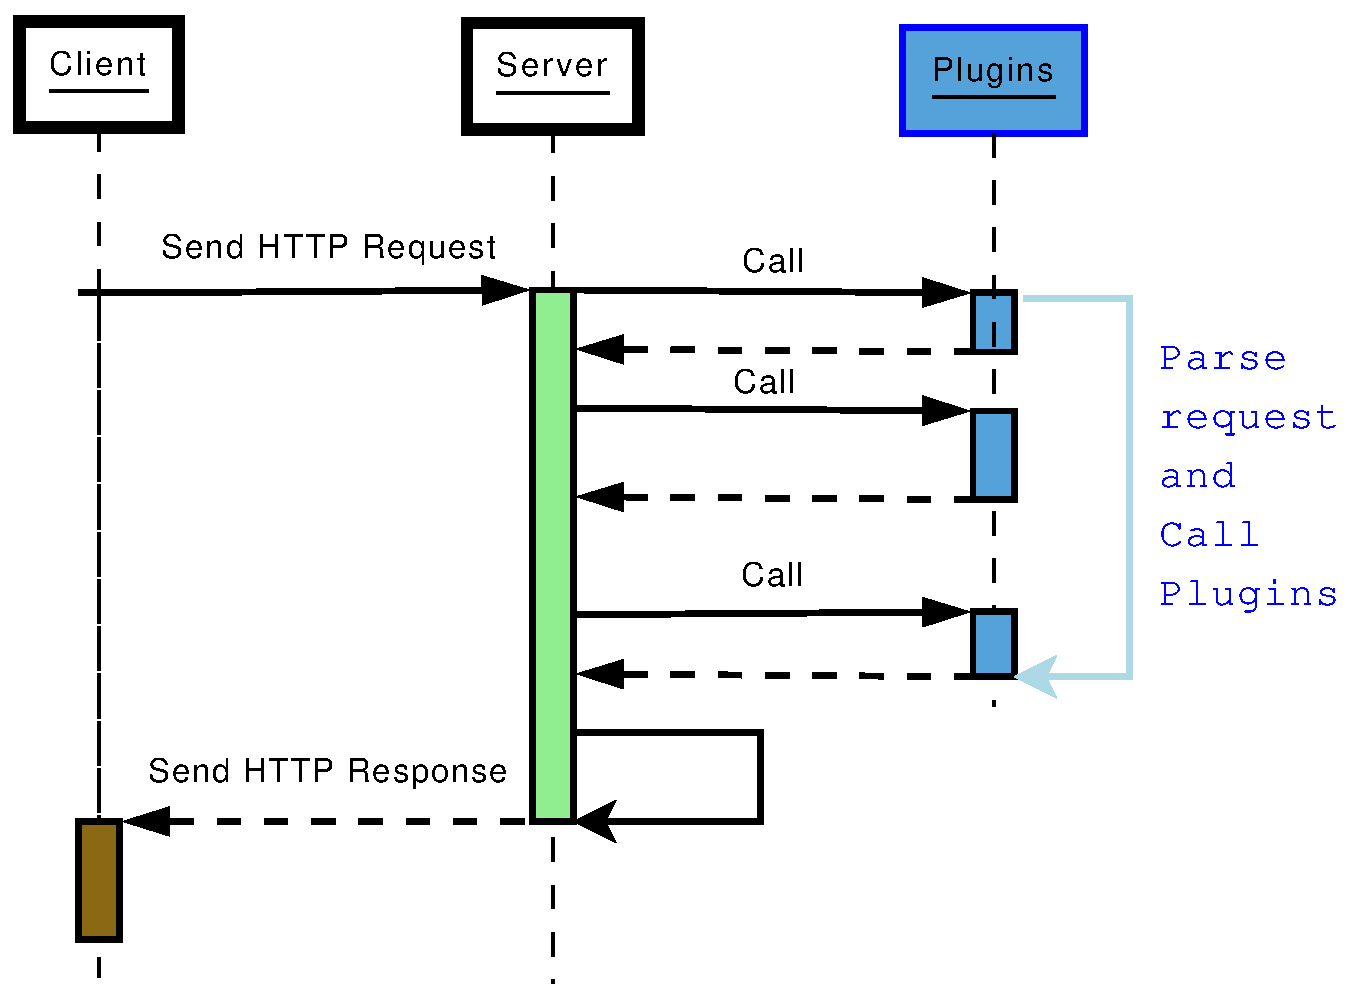
\includegraphics[height=5cm, width=8cm]{pics/httpplugin.eps}
	\caption{接口调用过程}
	\end{figure}

\end{frame}


\begin{frame}
	\frametitle{动态扩展功能接口定义:}
	接口定义了一些列函数原型。所有函数都有明确的定义和调用时机。
	
	功能插件选择性的实现这些函数。服务器在确定的时机调用所有插件的对应函数。
	
	\pause
	
	\begin{block}{接口函数定义:}
	\begin{itemize}
		\item[-] init: 初始化插件。
		\item[-] set\_default: 设置插件的配置为默认值。
		\item[-] cleanup: 清理插件。
		\item[-] trigger: 每秒钟调用一次。相当于计时器。
		\item[-] sighup: 处理挂断信号。
	\end{itemize}
	\end{block}
\end{frame}

\begin{frame}
	\frametitle{动态扩展功能接口定义:}
	\begin{block}{接口函数定义(续):}
	\begin{itemize}
		\item[-] url\_raw: 获得未解码的URL地址后调用。
		\item[-] url\_clean: 获得已解码的URL地址后调用。
		\item[-] docroot: 设置插件工作的根目录 。
		\item[-] physical: 获得请求资源对应的物理地址后调用。
		\item[-] connection\_close: 连接关闭时调用。
		\item[-] connection\_reset: 连接重置时调用。
		\item[-] joblist: 连接被加入joblist时调用嗯。
		\item[-] subrequest\_start: 子请求开始。
		\item[-] handle\_subrequest: 处理子请求。
		\item[-] subrequest\_end: 子请求结束。
	\end{itemize}
	\end{block}
\end{frame}


\begin{frame}
	\frametitle{动态加载过程}
	
	服务器实时的监测插件配置文件是否修改。一旦监测到修改,立即重新加载功能插件。

	\begin{figure}[htbp]
	\centering
	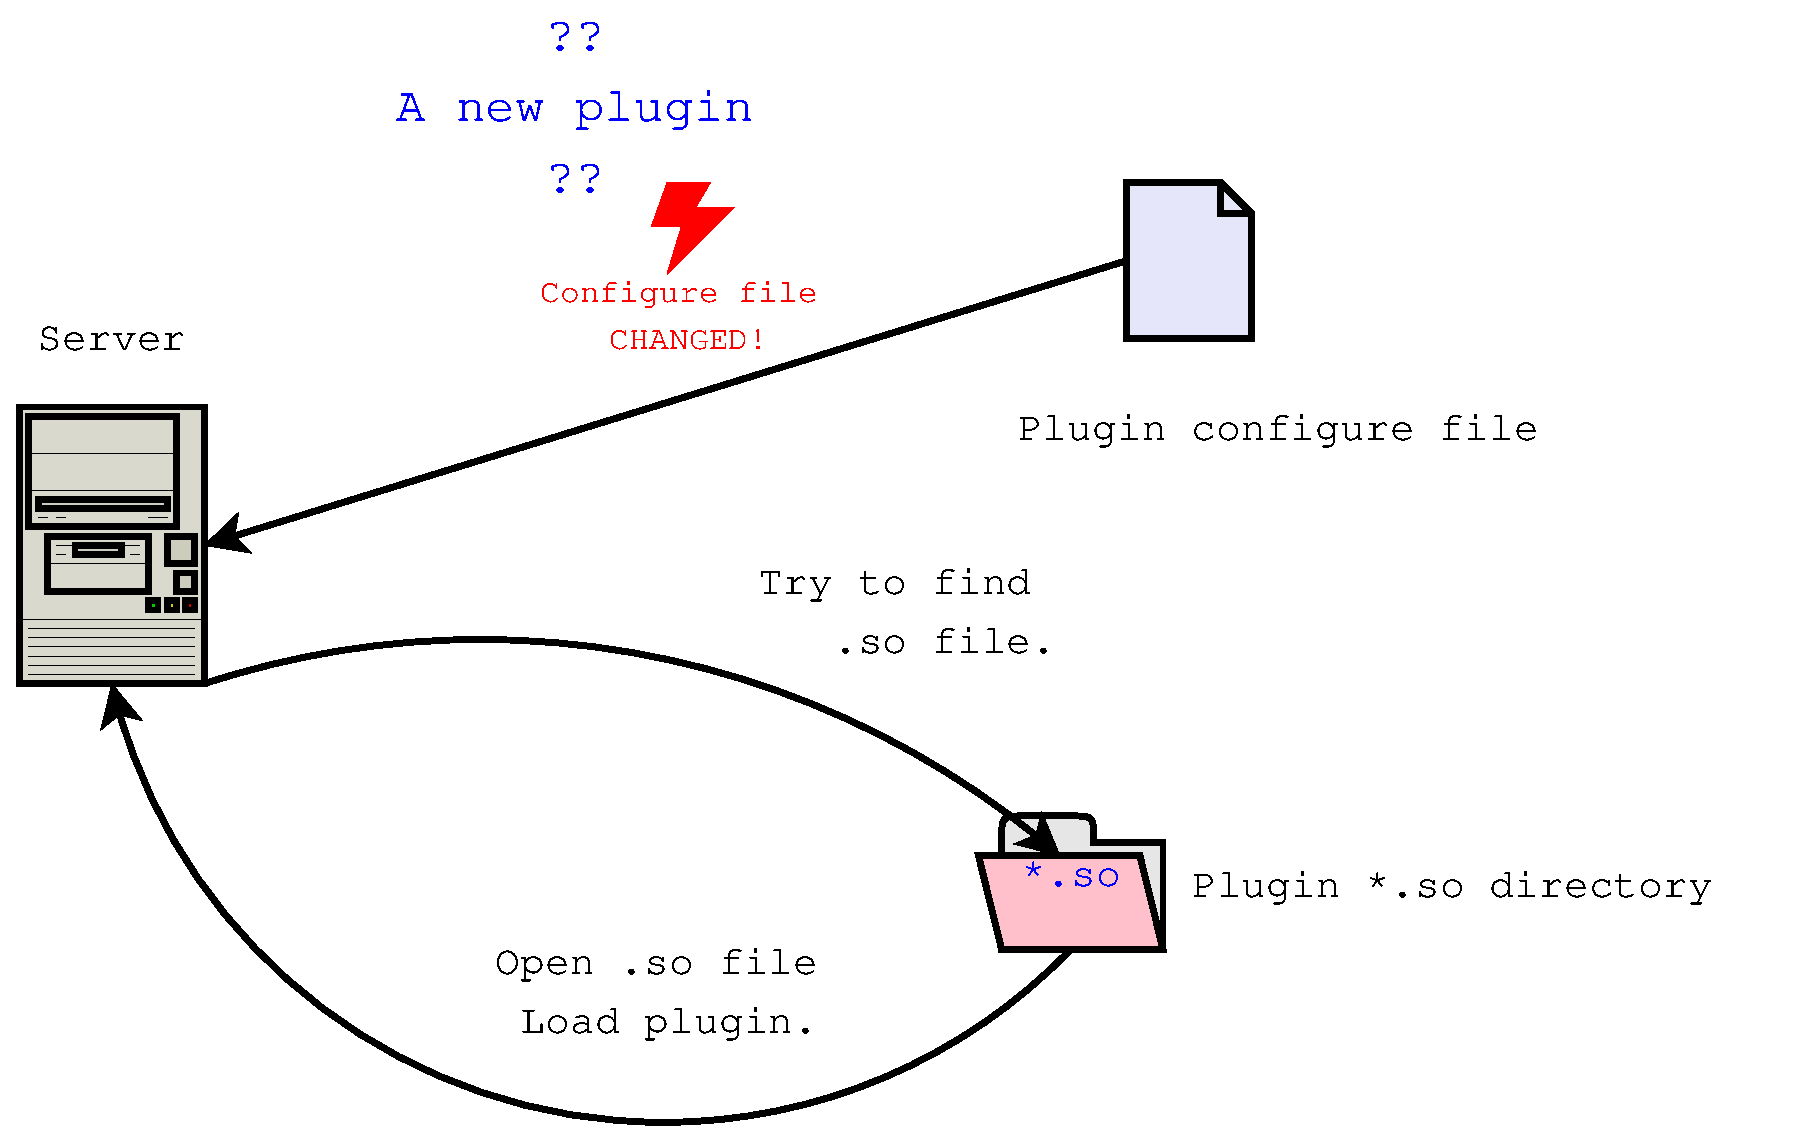
\includegraphics[height=5cm, width=9cm]{pics/loadplugin.eps}
	\caption{处理过程}
	\end{figure}

\end{frame}

\begin{frame}
	\frametitle{I/O分析和设计}
	\begin{columns}
		\begin{column}{0.25\textwidth}
			\begin{alertblock}{}
				Nonblocking IO
			\end{alertblock}
			
		\end{column}
		
		\begin{column}{0.02\textwidth}
			\begin{alertblock}{}
				+
			\end{alertblock}
		\end{column}
		
		\begin{column}{0.28\textwidth}
			\begin{alertblock}{}
				IO multiplexing
			\end{alertblock}
			
		\end{column}
		
		\begin{column}{0.02\textwidth}
			\begin{alertblock}{}
				+
			\end{alertblock}
		\end{column}
		
		\begin{column}{0.22\textwidth}
			\begin{alertblock}{}
				Thread pool
			\end{alertblock}
		\end{column}
	\end{columns}

	\begin{figure}[htbp]
	\centering
	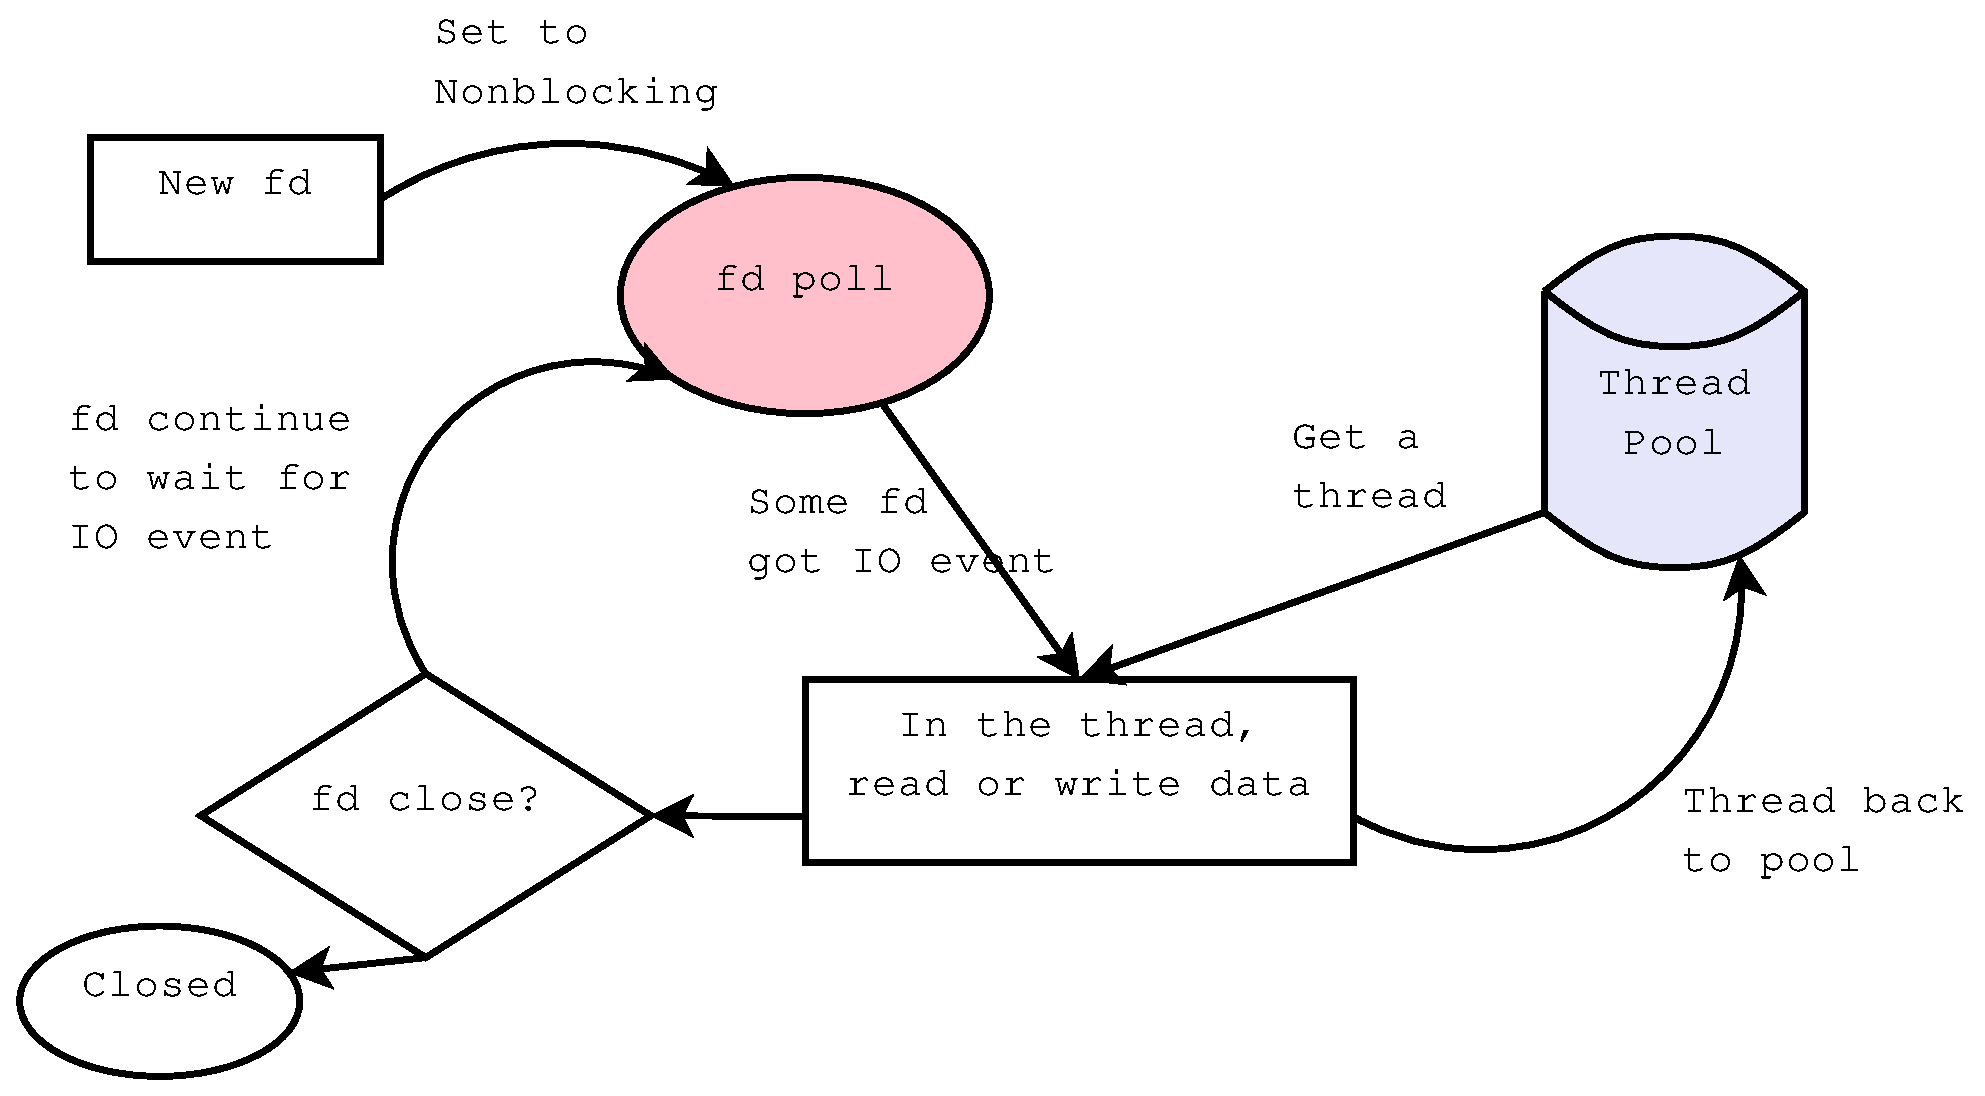
\includegraphics[height=5cm, width=10cm]{pics/IO.eps}
	\caption{I/O结构图}
	\end{figure}

	
\end{frame}


\begin{frame}
	\frametitle{状态机和线程池}
	\begin{block}{状态机}
	使用状态机对连接进行处理。
	
	对连接定义一系列状态。在整个生命周期中,连接处于某一个状态。根据连接的当前状态和所发生的事件,使连接进入下一状态。
	\end{block}
	\pause
	\begin{block}{线程池}
	每一个I/O事件调用一个线程进行处理。
	
	预先创建一部分线程。如果线程不够,再创建新的线程。线程处理完I/O事件不销毁,放入线程池中以备下次继续使用。
	
	降低线程创建和销毁的开销。
	\end{block}
\end{frame}

\section{动态扩展功能接口和服务器的实现}

\begin{frame}
	\frametitle{动态扩展功能接口和服务器的实现}
	\begin{center}
	{\Large
		三、动态扩展功能接口和服务器的实现
	}
	\end{center}
\end{frame}

\frame[containsverbatim]{
	\frametitle{接口实现:plugin结构体}
	
	plugin结构体包含一个插件的所有信息。包括版本,名称以及一系列接口函数的地址。plugin结构体类似于一个类。服务器通过调用其成员方法(函数指针)来执行插件的功能。
	
	定义如下:
	\begin{figure}[htbp]
	\centering
	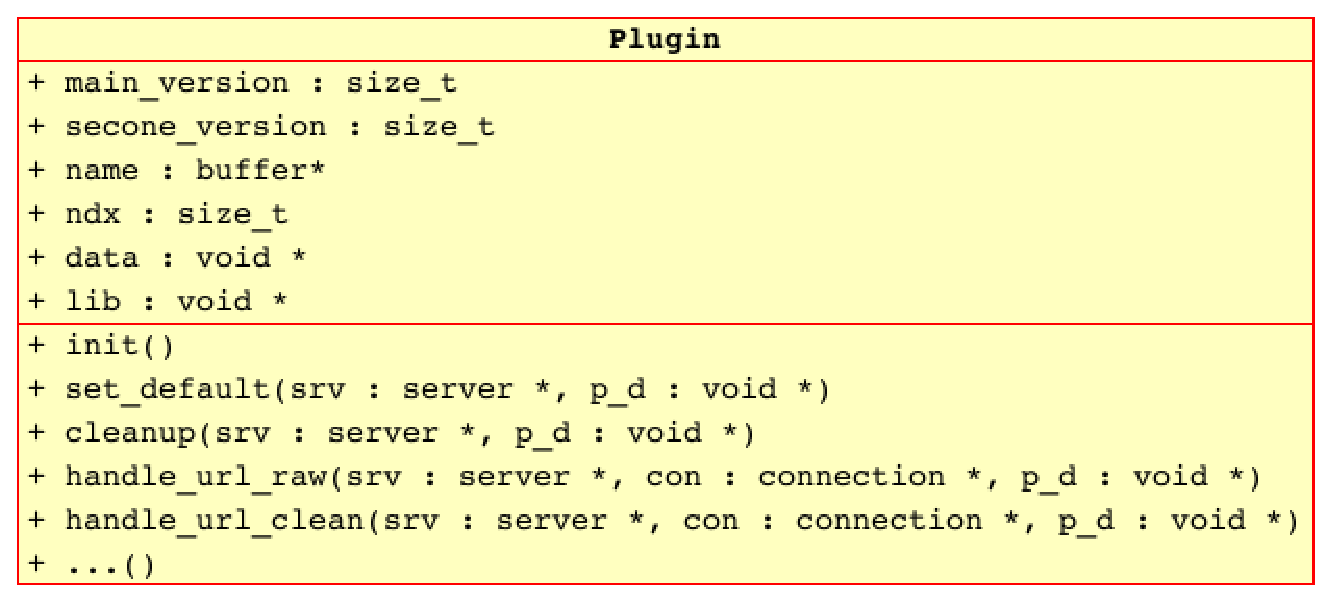
\includegraphics[height=4cm, width=8cm]{pics/plugin_s.eps}
	\caption{plugin结构体}
	\end{figure}
}


\begin{frame}
	\frametitle{接口实现:plugin\_slot数组}
	plugin\_slot是一个二维数组。相当于plugin的登记表。服务器通过这个表中的信息对插件进行调用。
	表的形式如下:
	\begin{table}[htbp]
	\caption{plugin\_slot示例:}
	\centering
	\begin{tabular}{cccc} %最后一列是空的。这样可以是倒数第二列居中,否则会报错或不居中。
	\toprule
	\centering 名称 & 插件1 & 插件2 &插件3\\
	\midrule
	\centering PLUGIN\_SLOT\_URL\_RAW & p1 &  p2 & p3\\
	\centering PLUGIN\_SLOT\_URL\_CLEAN &  p1 &  NULL & p3\\
	\centering PLUGIN\_SLOT\_DOCROOT & p1 & NULL & NULL\\
	\bottomrule
	\end{tabular}
	\end{table}
	\begin{block}{}
		表中存放的是plugin结构体指针。NULL表示此插件没有实现这个函数。
	\end{block}
\end{frame}

\begin{frame}
	\frametitle{接口实现}
	服务器中包含一个定义插件的配置文件: swiftd-plugin.conf。
	
	\begin{block}{配置文件的形式如下:}	
		\#swiftd-plugin.conf
		\#配置文件的形式为  -- 插件名称:插件动态库文件所在目录\$\\
		\#每个插件一行,每个插件配置信息必须以"\$"结尾。\\
		dir\_index:/home/hcy/plugins/\$\\
		...
	\end{block}
	
	\pause
	
	\begin{block}{}
	动态库文件的名称为: \textcolor{red}{插件名称 + .so}。\\
	服务器通过监测这个配置文件,确定是否有插件需要加载或删除。
	\end{block}
\end{frame}

\begin{frame}
	\frametitle{接口实现}
	服务器使用inotify监测插件配置文件。inotify产生一个文件描述符,通过监测这个文件描述符是否有数据可读即可监测到文件的改变。
	\begin{figure}[htbp]
	\centering
	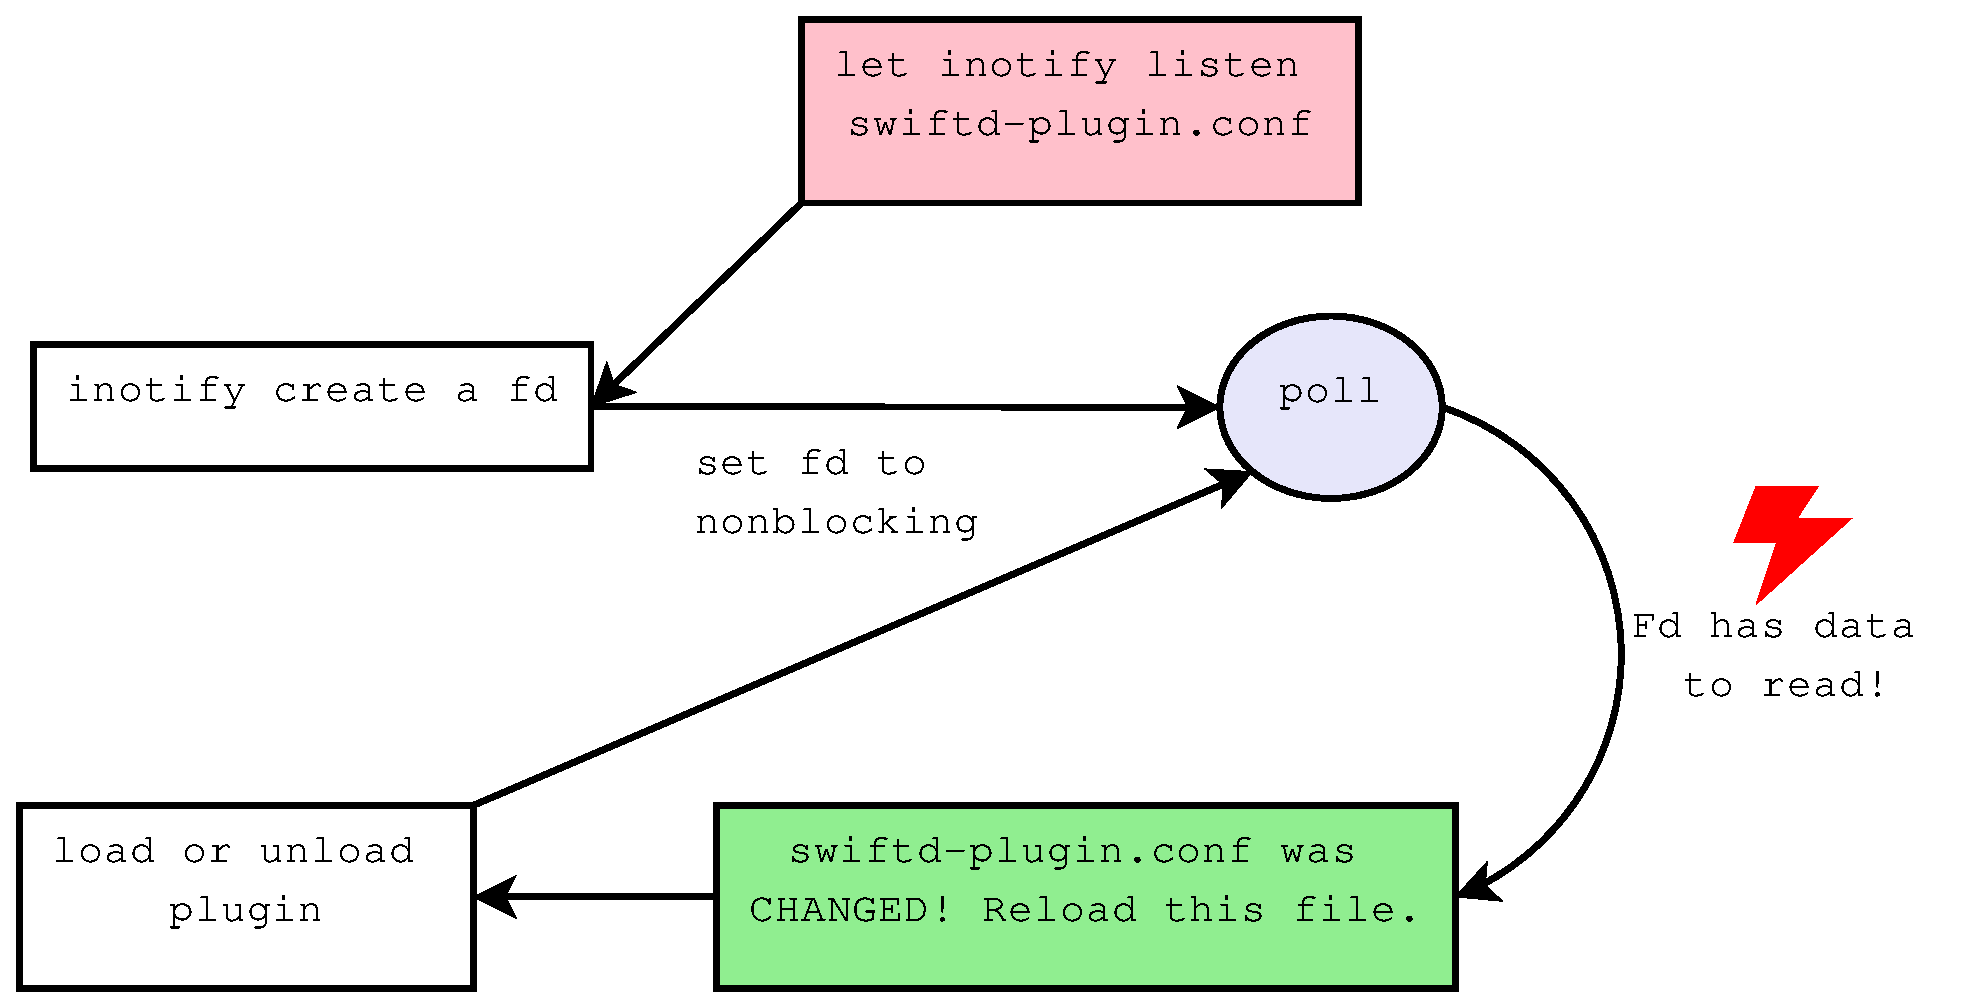
\includegraphics[height=5cm, width=9cm]{pics/inotify.eps}
	\caption{监测的过程}
	\end{figure}
\end{frame}

\begin{frame}
	\frametitle{服务器实现}
	\begin{block}{I/O}
	使用epoll对文件描述符的IO事件进行监测。
	
	epoll的效率高于select/poll。
	\end{block}
	%每个文件描述符都有一个对应的IO事件处理函数。一旦有IO事件发生,申请一个线程,在线程中调用这个函数处理IO事件。
	
	\pause
	\begin{block}{线程池}
		每个线程的主循环中,调用传递进来的函数。(包括参数)\\
		使用pthread的条件变量对线程进行唤醒和睡眠操作。\\
		预先创建线程。提高效率。
	\end{block}
	
	\pause
	\begin{block}{状态机}
	对于每个连接,在其生存周期中,共定义了11个状态。包括connection,requeststart,read,handlerequest, \\requestend,readpose,responsestart,write,responseend,\\error和close。
	\end{block}
\end{frame}

\begin{frame}
	\begin{columns}
	\frametitle{连接处理状态机}
	
	\begin{column}{0.6\textwidth}
		\begin{figure}[htbp]
		\centering
		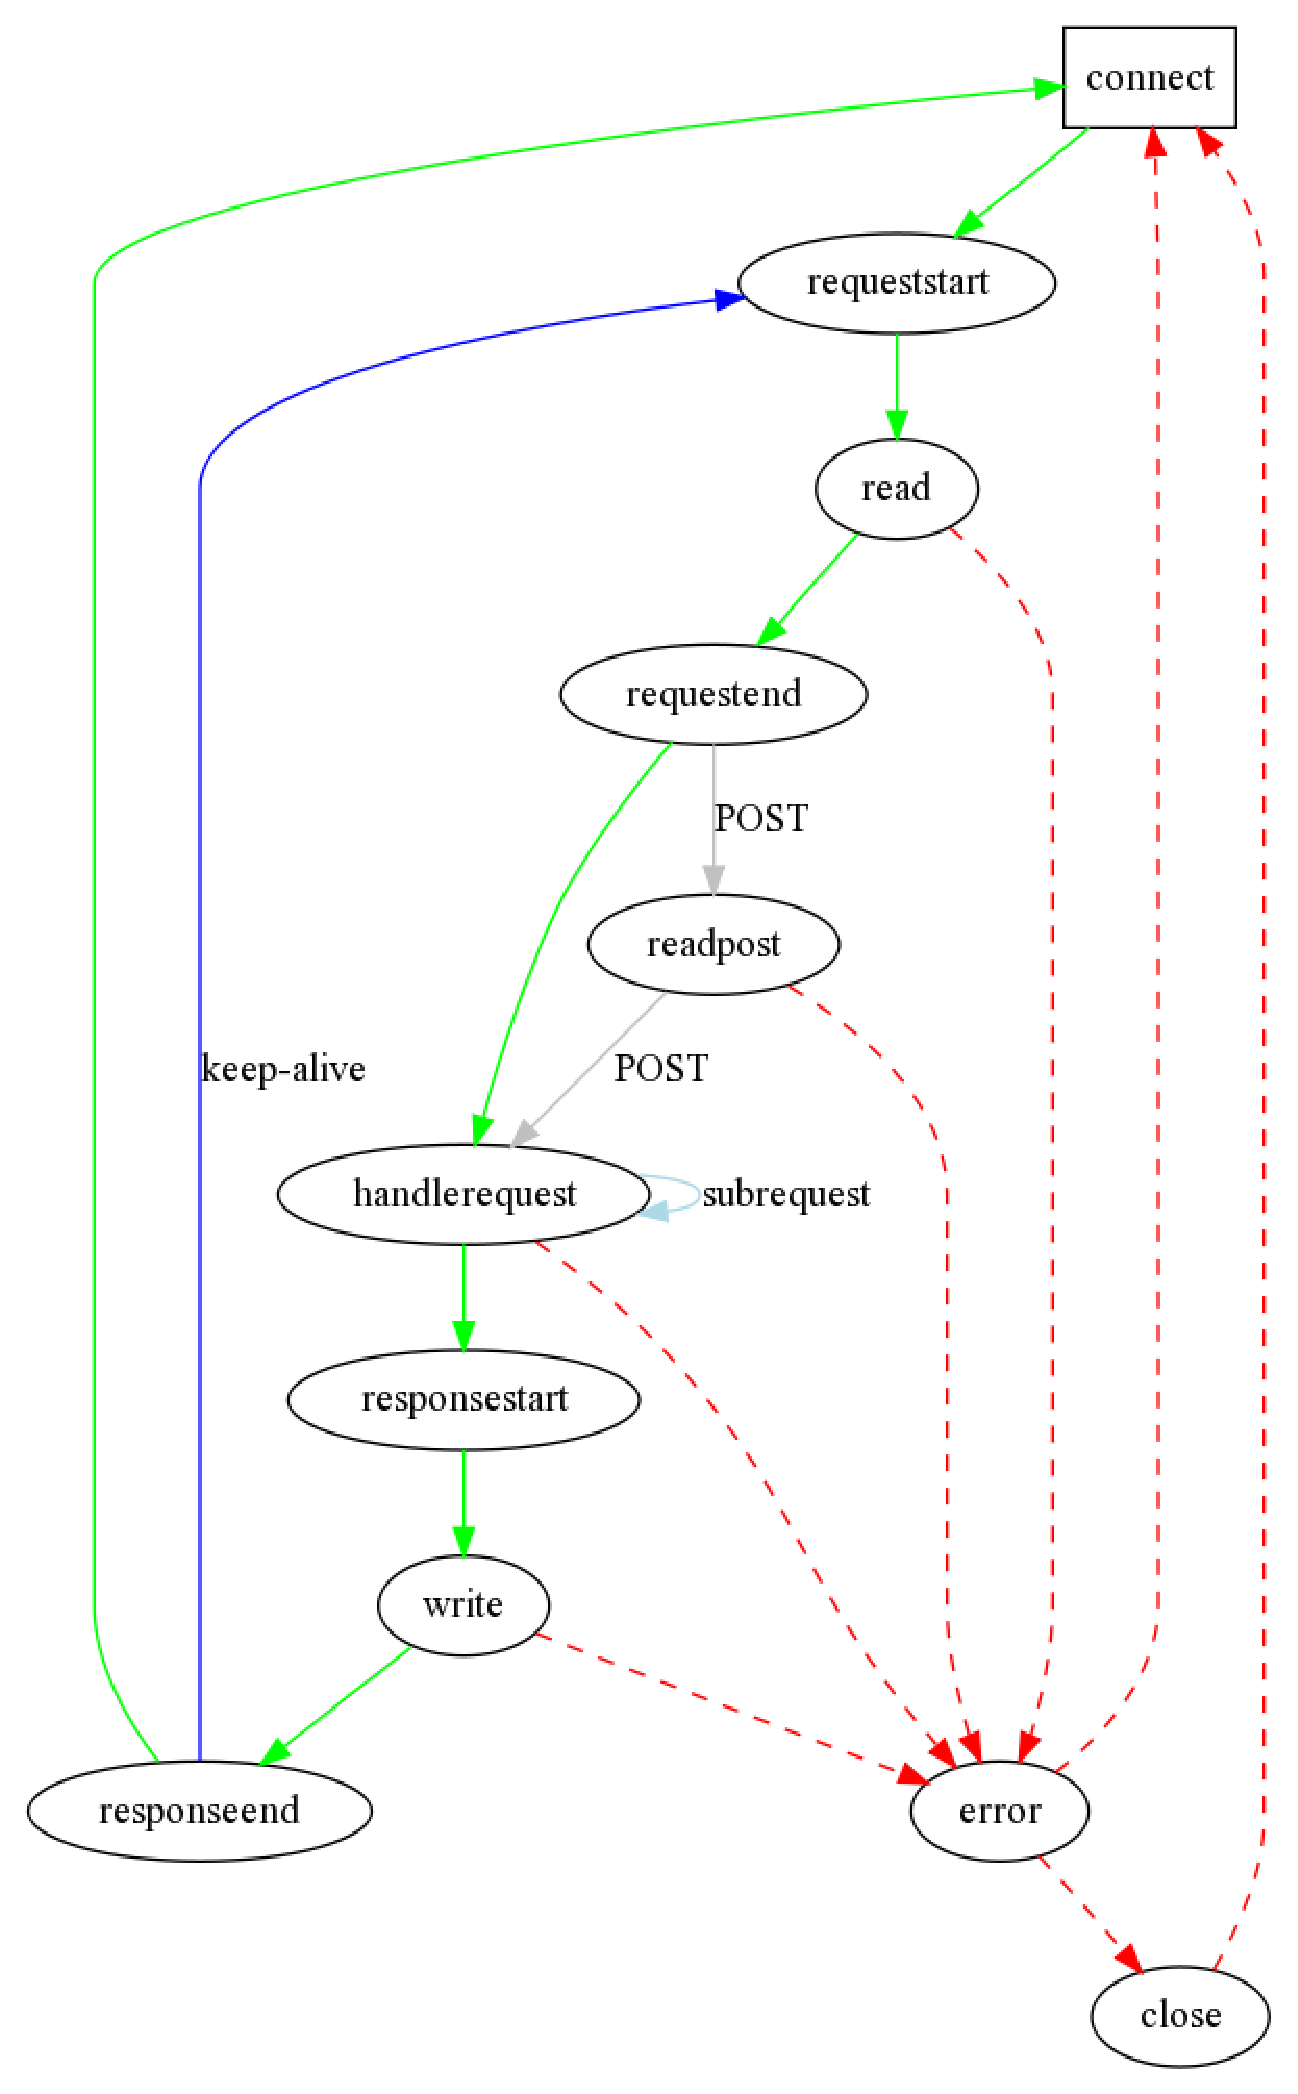
\includegraphics[height=7.5cm, width=6cm]{pics/state.eps}
		\end{figure}
	\end{column}
	
	\begin{column}{0.3\textwidth}
		\begin{block}{}
			\textcolor{green}{绿色路径}为一个正常的处理路径。\\
		\end{block}
		\begin{block}{}
			\textcolor{red}{红色路径}为出错路径。\\
		\end{block}
		\begin{block}{}	
			\textcolor{blue}{蓝色路径},HTTP/1.1中保持连接。
		\end{block}
	\end{column}
	
	\end{columns}
	
\end{frame}

\section{运行结果}
\begin{frame}
	\frametitle{运行结果}
	\begin{center}
	{\Large
		四、运行结果
	}
	\end{center}
\end{frame}

\begin{frame}
	\frametitle{启动和访问}
	\begin{columns}
		\begin{column}{0.4\textwidth}
			启动:
			\begin{figure}[htbp]
			\centering
			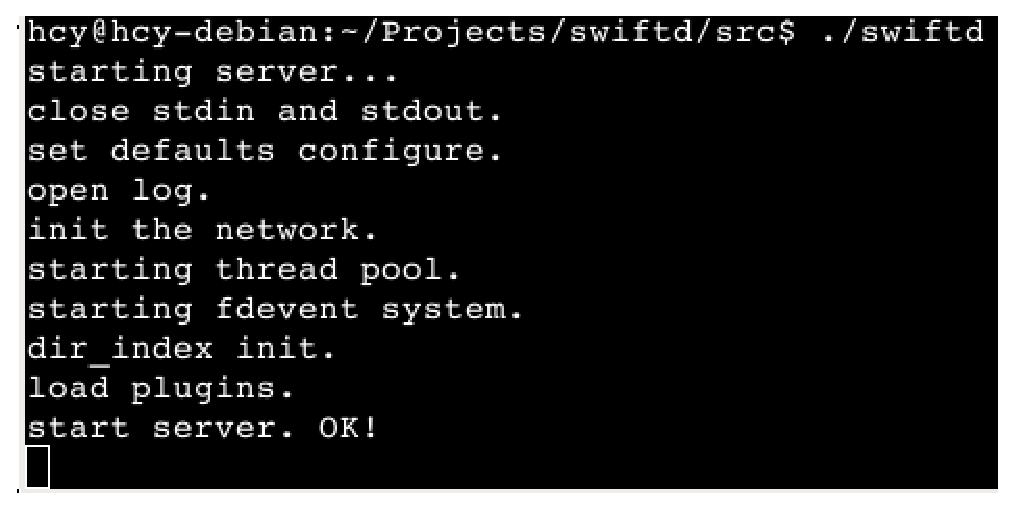
\includegraphics[height=3cm, width=4.5cm]{pics/startup.eps}
			\end{figure}
		\end{column}
		
		\begin{column}{0.5\textwidth}
			正常访问
			\begin{figure}[htbp]
			\centering
			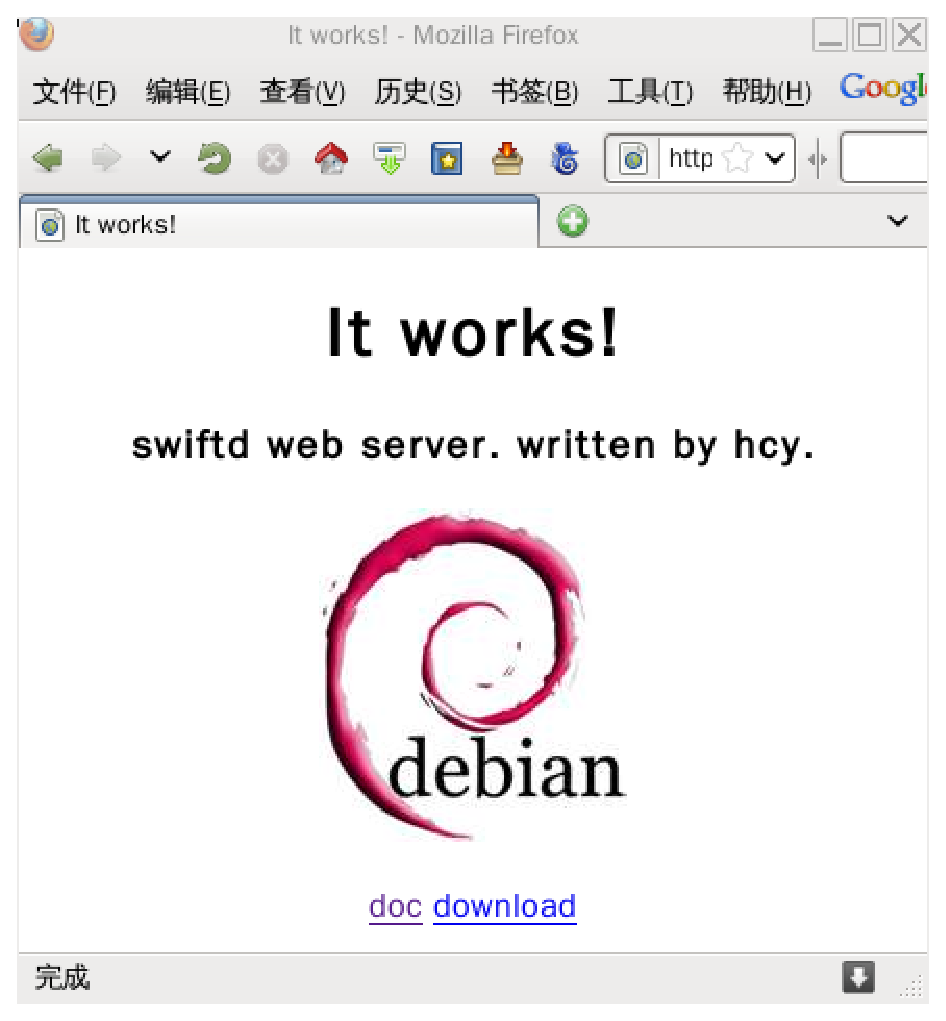
\includegraphics[height=5cm, width=6cm]{pics/works.eps}
			\end{figure}

		\end{column}
	\end{columns}
\end{frame}

\begin{frame}
	\frametitle{运行结果}
	\begin{columns}
		\begin{column}{0.6\textwidth}
			注释掉插件配置:
			\begin{figure}[htbp]
			\centering
			
\includegraphics[height=3cm, width=4.5cm]{pics/complugin.eps}
			\end{figure}
		\end{column}
		
		\begin{column}{0.3\textwidth}
			\textcolor{red}{服务器不需要重启!}
		\end{column}
	\end{columns}
	
	访问失败:
	\begin{figure}[htbp]
	\centering
	
\includegraphics[height=2.5cm, width=6cm]{pics/nodirindex.eps}
	\end{figure}
\end{frame}

\begin{frame}
	\frametitle{运行结果}
	\begin{columns}
		\begin{column}{0.6\textwidth}
			增加插件配置:
			\begin{figure}[htbp]
			\centering
			
\includegraphics[height=3cm, width=4.5cm]{pics/uncomplugin.eps}
			\end{figure}
		\end{column}
		
		\begin{column}{0.3\textwidth}
			\textcolor{green}{服务器同样不需要重启!}
		\end{column}
	\end{columns}
	
	访问成功:
	\begin{figure}[htbp]
	\centering
	
\includegraphics[height=2.5cm, width=7cm]{pics/dirindex.eps}
	\end{figure}

\end{frame}

\section{总结}
\begin{frame}
	\frametitle{总结}
	\begin{center}
	{\Large
		五、总结
	}
	\end{center}
\end{frame}

\begin{frame}
	\frametitle{运行结果}
	\begin{enumerate}
		\item 阅读关于HTTP协议的相关资料,理解了HTTP协议的处理过程。
		\item 学习了在Linux下进行开发。熟悉了linux,gcc,gdb,vim等的使用。
		\item 动态加载功能接口达到了课题的目标要求。可以正确的进行动态加载和卸载功能插件。
		\item 服务器可以正确处理HTTP请求。包括HTTP/1.1和HTTP/1.0。能够正确的调用插件处理请求。
		\item 总共完成11000行C代码的编写和调试。
	\end{enumerate}
\end{frame}

\begin{frame}
	\frametitle{结束}
	\begin{center}
	{\Huge
		That's all!
	}
	\end{center}
\end{frame}

\end{document}
